\documentclass[10pt,dvipsnames]{beamer}
\usepackage{amsmath,amssymb,longtable,hhline}
\usepackage{mathrsfs}
\usepackage{xcolor}
\usepackage{hyperref}
\usepackage{multicol}
\usepackage{anyfontsize}
\usepackage{minted}

\usemintedstyle{tango}
\newcommand{\ltprgsize}{\fontsize{5}{5}\selectfont}
\setminted{fontsize=\ltprgsize,mathescape}

\definecolor{mygreen}{rgb}{0,0.6,0}
\definecolor{mygray}{rgb}{0.5,0.5,0.5}
\definecolor{mymauve}{rgb}{0.58,0,0.82}

\hypersetup{
    bookmarks=true,         % show bookmarks bar?
    unicode=true,           % non-Latin characters in Acrobat’s bookmarks
    pdftoolbar=false,        % show Acrobat’s toolbar?
    pdfmenubar=false,        % show Acrobat’s menu?
    pdffitwindow=false,     % window fit to page when opened
    pdfstartview={FitH},    % fits the width of the page to the window
    pdftitle={Компьютерная алгебра в задачах оптимизации},    % title
    pdfauthor={Evgeny Cherkashin, Seseg Badmatsyrenova},     % author
    pdfsubject={symbolic computations},   % subject of the document
    pdfnewwindow=true,      % links in new PDF window
    colorlinks=true,       % false: boxed links; true: colored links
    linkcolor=red,          % color of internal links (change box color with linkbordercolor)
    citecolor=green,        % color of links to bibliography
    filecolor=magenta,      % color of file links
    urlcolor=blue           % color of external links
}

\usepackage{pifont}

\usetheme{Warsaw}
\usecolortheme{crane}
%\useinnertheme{rectangles}
\setbeamertemplate{itemize item}{\scriptsize\hbox{\donotcoloroutermaths\ding{113}}}
\setbeamertemplate{itemize subitem}{\tiny\raise1.5pt\hbox{\donotcoloroutermaths$\blacktriangleright$}}
\setbeamertemplate{itemize subsubitem}{\tiny\raise1.5pt\hbox{\donotcoloroutermaths$\blacktriangleright$}}
\setbeamertemplate{enumerate item}{\insertenumlabel.}
\setbeamertemplate{enumerate subitem}{\insertenumlabel.\insertsubenumlabel}
\setbeamertemplate{enumerate subsubitem}{\insertenumlabel.\insertsubenumlabel.\insertsubsubenumlabel}
\setbeamertemplate{enumerate mini template}{\insertenumlabel}

\beamertemplatenavigationsymbolsempty

\usepackage{iftex,ifxetex}
\ifPDFTeX
  \usepackage[utf8]{inputenc}
  \usepackage[T1]{fontenc}
  \usepackage[russian]{babel}
  \usepackage{lmodern}
  \usefonttheme{serif}
\else
  \ifluatex
    \usepackage{unicode-math}
    \defaultfontfeatures{Ligatures=TeX,Numbers=OldStyle}
    \setmathfont{Latin Modern Math}
    \setsansfont{Linux Biolinum O}
    \setmonofont{Fira Mono}
    \usefonttheme{professionalfonts}
    % \setmathfont[
    %     Ligatures=TeX,
    %     Scale=MatchLowercase,
    %     math-style=upright,
    %     vargreek-shape=unicode
    %     ]{euler.otf}
  \fi
\fi

%\useoutertheme{split}
%\useinnertheme{rounded}
\setbeamertemplate{background canvas}[vertical shading][bottom=white!80!cyan!20,top=cyan!10]
%\setbeamertemplate{sidebar canvas left}[horizontal shading][left=white!40!black,right=black]

\graphicspath{{pics/}}


% --------------------------

\def\remph#1{\textcolor{Mahogany}{\bfseries #1}}

\begin{document}
\parindent=1em
\title{Recommender systems for career guidance}
\author{
\def\and{, }
Trần Đức Thế\and
\remph{Evgeny~Cherkashin}\and
Viktoria Kopylova\and
Nikita Lukyanov}


\date{${}$\\\vspace{2em}AIIT-2021, October, 15}
\institute{\textit{Matrosov Institute for System Dynamics and Control Theory of SB RAS}, Irkutsk, Russia,
  \href{mailto:eugeneai@icc.ru}{eugeneai@icc.ru}\\
  \textit{National research Irkutsk state technical university,} Irkutsk, Russia,
  \href{mailto:kopylovika@mail.ru}{kopylovika@mail.ru}}

\maketitle
% ----------------------------------------------------------------
\begin{frame}{Introduction}

  \emph{Recommender systems} (RS) are examples of \emph{decision support systems}. They are useful to support users with additional information and decision variants.  We consider two RS in career guidance field.

Both systems were developed within master degrees at Institute for Information Technologies and Data Analysis, National research Irkutsk state technical university.

\textbf{Relevance} is determined by
\begin{itemize}
\item In the countries with young population, such as Việt Nam, the demand of young specialists is high. In fact, quite often graduates remain unemployed for a long time or do not work in originally mastered specialties.
\item University institutions are interested in rising quality of entrants: attract attention of domain targeted students with high potentials to the existing courses, organize new courses for target student groups.
\end{itemize}

%In the \textbf{second} RS entrants are to obtain perspective specialty, comfort to their nature.  There are no industry supporting career guidance, only informational services and neighbors' subjective experience.  The universities' activities should be focused to a target audience with supplying students \textbf{relevant optional courses}.


\end{frame}

\begin{frame}
  \frametitle{Interest assessment}
  In Tables 1 and 2, we present the result of interest assessment to career guidance and relevance of improving of the guidance system.
\begin{table}[thb]
  \caption{Interest assessment to the carer guidance in Việt Nam, Hà Tĩnh city}
  \label{tab:interest}
  \centering
  \begin{tabular}{|l|c|c|}
    \hline
    \textbf{Interest level} & \textbf{Count of votes} & \textbf{Ratio, \%} \\
    \hline
    Very interested & 218 & 51.9 \\
    \hline
    Relatively interested & 155 & 36.9 \\
    \hline
    Less interested & 36 & 8.6 \\
    \hline
    No interest & 11 & 2.6 \\
    \textbf{Total} & 420 & 100 \\
    \hline
  \end{tabular}
\end{table}

\begin{table}[bht]
  \caption{Questionary results of middle school students on need for improvement of the carer guidance system}
  \label{tab:interest}
  \centering
  \begin{tabular}{|l|c|c|}
    \hline
    \textbf{Answer option} & \textbf{Quantity} & \textbf{Ration, \%} \\
    \hline
    very necessary & 272 & 64.8 \\
    \hline
    necessary & 145 & 34.5 \\
    \hline
    no necessity & 3 & 0.7 \\
    \hline
    \texttt{Total} & 420 & 100 \\
    \hline
  \end{tabular}
\end{table}
\end{frame}

\begin{frame}
  \frametitle{Ralated Works Summary}
  The \emph{collaborative filtration} is currently more popular than \emph{content filtering} as it allows one to solve ``\textbf{cold start}'' problem: initial lack of information and interest transformations due to modern trends.
  \begin{itemize}
  \item Real estate RS sometimes attract sellers to be the experts for content filtering;
  \item Spacial data of realty surroundings are estimated;
  \item Problem stated in game and control theory domains (satisfy the most customers);
  \item Reflect entrants GCE grades to a specialty, predicting univ. grades;
  \item Forecast learning trajectories of students by similarity to graduate ones;
  \item Advice students with a course, analyzing text descriptions of courses;
  \end{itemize}

  We aim at application of known techniques to the source data of Irkutsk region.
\end{frame}

\begin{frame}
  \frametitle{Preliminary data processing: Real Estate RS}
  Real estate (RE) \textbf{objects} are presented at \emph{classified advertisement websites} and special RE ones \texttt{altcom.ru} storing \emph{offers}.  Offers refer RE objects described by properties (address, sizes, levels, number of rooms, etc.).  Input format is XML, being essentially a list.

  RE \textbf{agents} have roles: \emph{unknown, seller, buyer, owner, realtor, expert, invalid user}.  Experts and realtors are RS managers.  The first three are regular users able to look for an object.

  Objects are distributed by hierarchical cluster analysis to classes: {\color{JungleGreen}two-room flats}, {\color{Melon}one-or-two-room flats} (comfort class realty), {\color{RawSienna}one-room flats}, {\color{Periwinkle}dachas}, {\color{ForestGreen}houses}, {\color{Mahogany}rooms}, {\color{Dandelion}commercial space}, {\color{Plum}a garage}, and {\color{MidnightBlue}elite realty} (flats with three and more rooms).  Naming is performed by \texttt{experts}.

  \textbf{User interest} is acquired by tracking his/her activity on web site. If user spent more than 30 seconds viewing an object data add a positive interest unit.  After some time user is suggested to register to provide cross-browser data acquisition.
\end{frame}

\begin{frame}
  \frametitle{Classification of Realty Objects}

 \begin{columns}
    \begin{column}{0.8\linewidth}
\begin{table}[tb]
  \footnotesize
  \centering
  \begin{tabular}{|l|l|c|c|}
    \hline
    Attribute & Calculation technique & $v_k, \%$ & Formula \\
    \hline
\texttt{string Name} & not used & & \\
    \texttt{ILocation Location} & equality & 10 & $(1)$
    \\
\texttt{string Address} & --''-- & 10 & \\
\texttt{float Price} & relative difference & 25 & $(2)$\\
\texttt{float Area} & relative difference  & 35 & $(2)$\\
\texttt{string ImageURL} & --''-- & & \\
\texttt{string URL} & --''-- & & \\
\texttt{int Rooms}  & relative difference  & 100 & $(2)$\\
\texttt{int RoomsOffered} &  --''--   & 100 & $(2)$\\
\texttt{int Floor}  &  --''--   & 30 & $(2)$\\
\texttt{int FloorTotal}  &  --''--   & 10 & $(2)$\\
\texttt{BuildingEnum \ldots}  & equality & 30 & $(1)$\\
\texttt{IBuilding \ldots{}}  & --''-- & 30 &  $(1)$\\
\texttt{PropertyEnum \ldots} & --''-- & 30 &  $(1)$\\
\texttt{CategoryEnum \ldots} & --''-- & 100 &  $(1)$\\
    \texttt{string GUID} & --''-- & & \\
    \hline
  \end{tabular}
  \end{table}
 \end{column}
\begin{column}{0.2\linewidth}\footnotesize
\[
  d_k(i,j) =
\]
\[
 =\left\{
                                                          \begin{array}{ll}
                                                            0, & \mbox{if\ \ } a_i=a_j,\\
                                                            1, & \mbox{if\ \ } a_i\neq a_j,
                                                          \end{array}
                                                        \right.
                                                      \]
                                                  \[
  (1)
\]
\\[2em]
\[
  = \frac{|a_i^k-a_j^k|}{a_i^k+a_j^k},\] \[ a_i^k+a_j^k>0.
  \quad (2)
\]
\end{column}
\end{columns}
\vspace{-1em}
\[
 \text{Reduction:}\qquad d(i,j)=\frac{\sum\limits_{k=1}^m|v_k\cdot d_k(i,j)|}{\sum\limits_{k=1}^m v_k}, \qquad 0\leqslant d_{i,j}\leqslant 1.
\]
%\noindent where $v_k$ is a weight of $k$-th attribute value, defined in the table.

\end{frame}

\begin{frame}
  \frametitle{Recommendations generation behavior}

   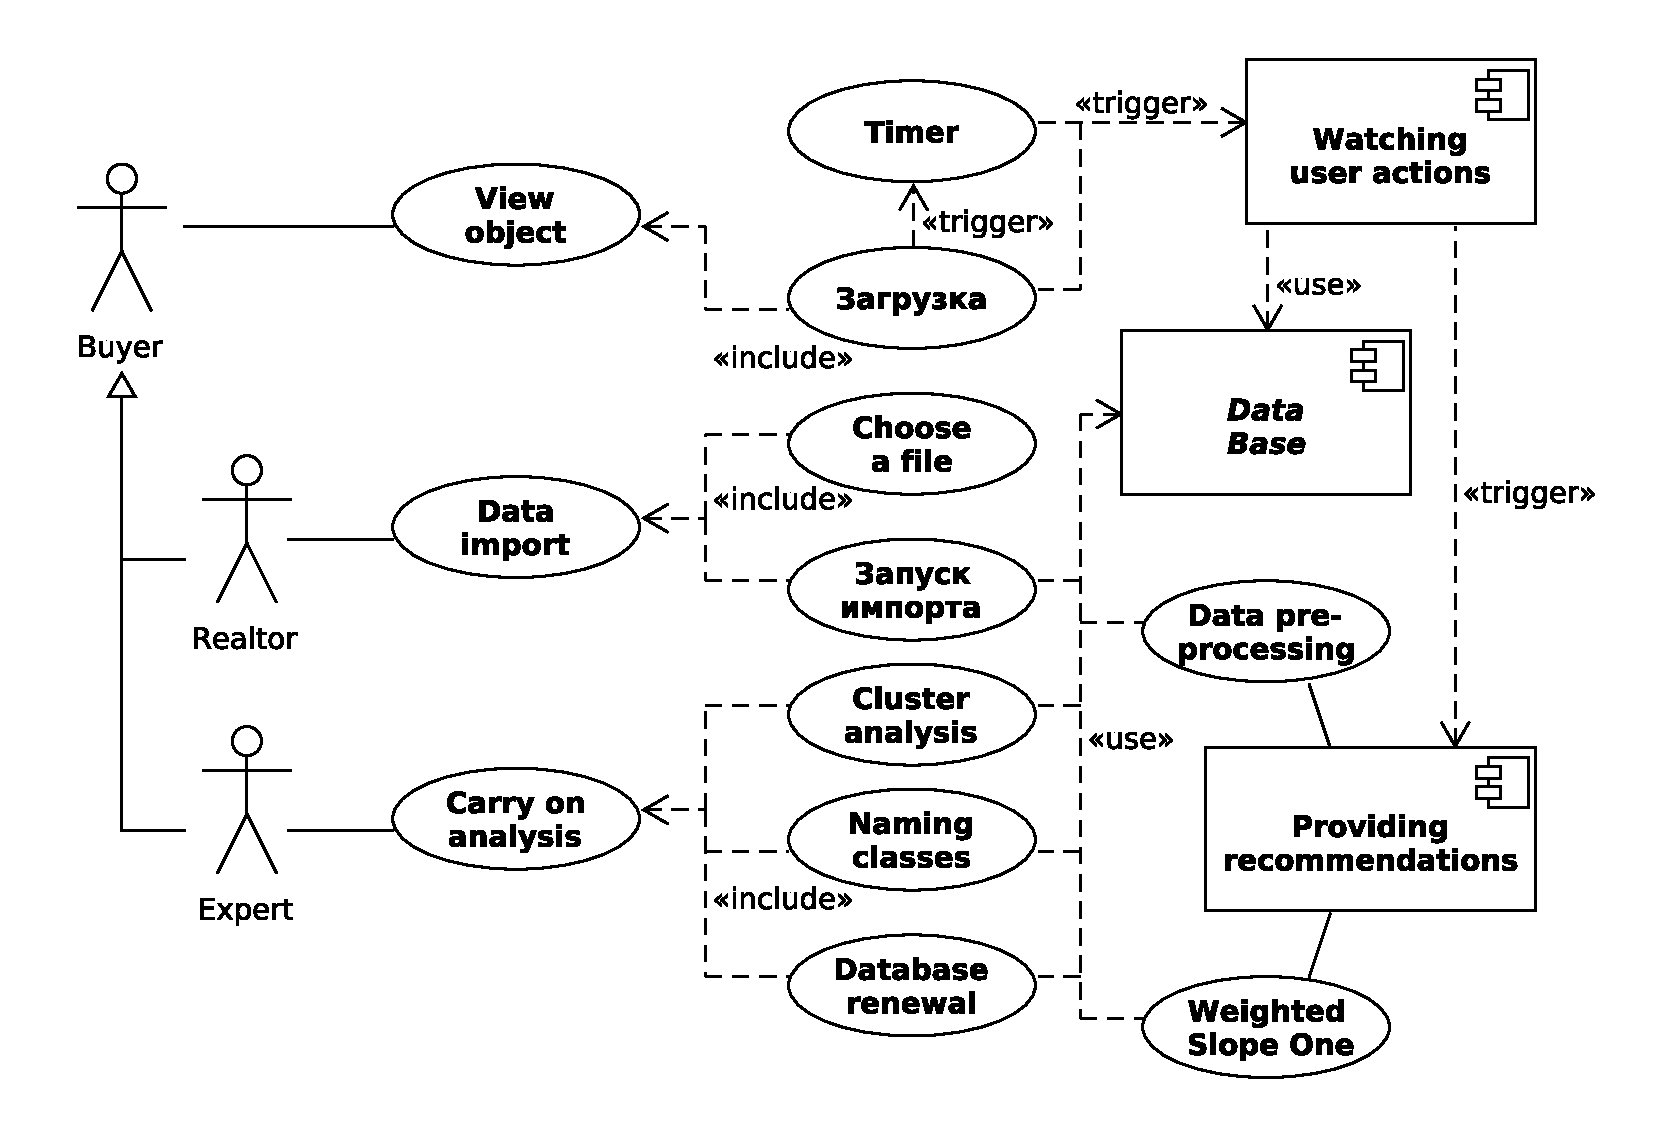
\includegraphics[width=1\linewidth]{use_case.eps}

\end{frame}

\begin{frame}
  \frametitle{Web Application}
  As the software platform of the RS is C\# we used ASP.NET based frameworks, such as \texttt{Nancy}, mapping an URL to a lambda function of one argument.

  HTTP template engine is based on SharpTAL, allowing implementation of MVC with a dictionary variable substitution.  It can be extended to support LOD cross-site integration.
\vfill\centering
  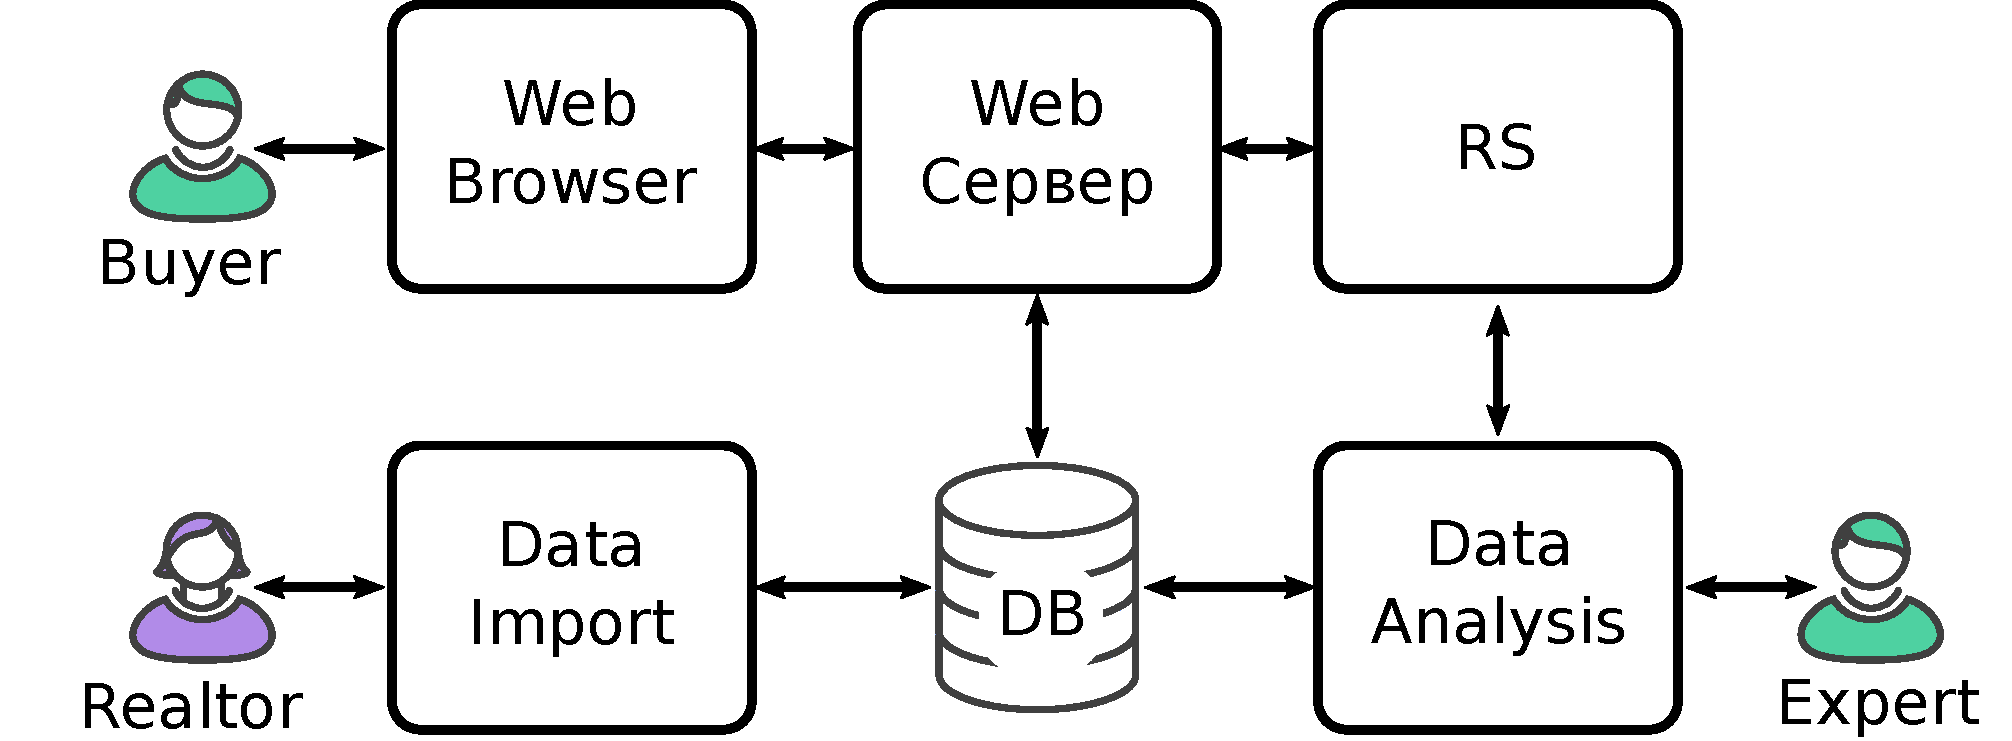
\includegraphics[width=1\linewidth]{architecture.pdf}
\end{frame}

\begin{frame}
  \frametitle{Persistent Object Structure}
   \centering
   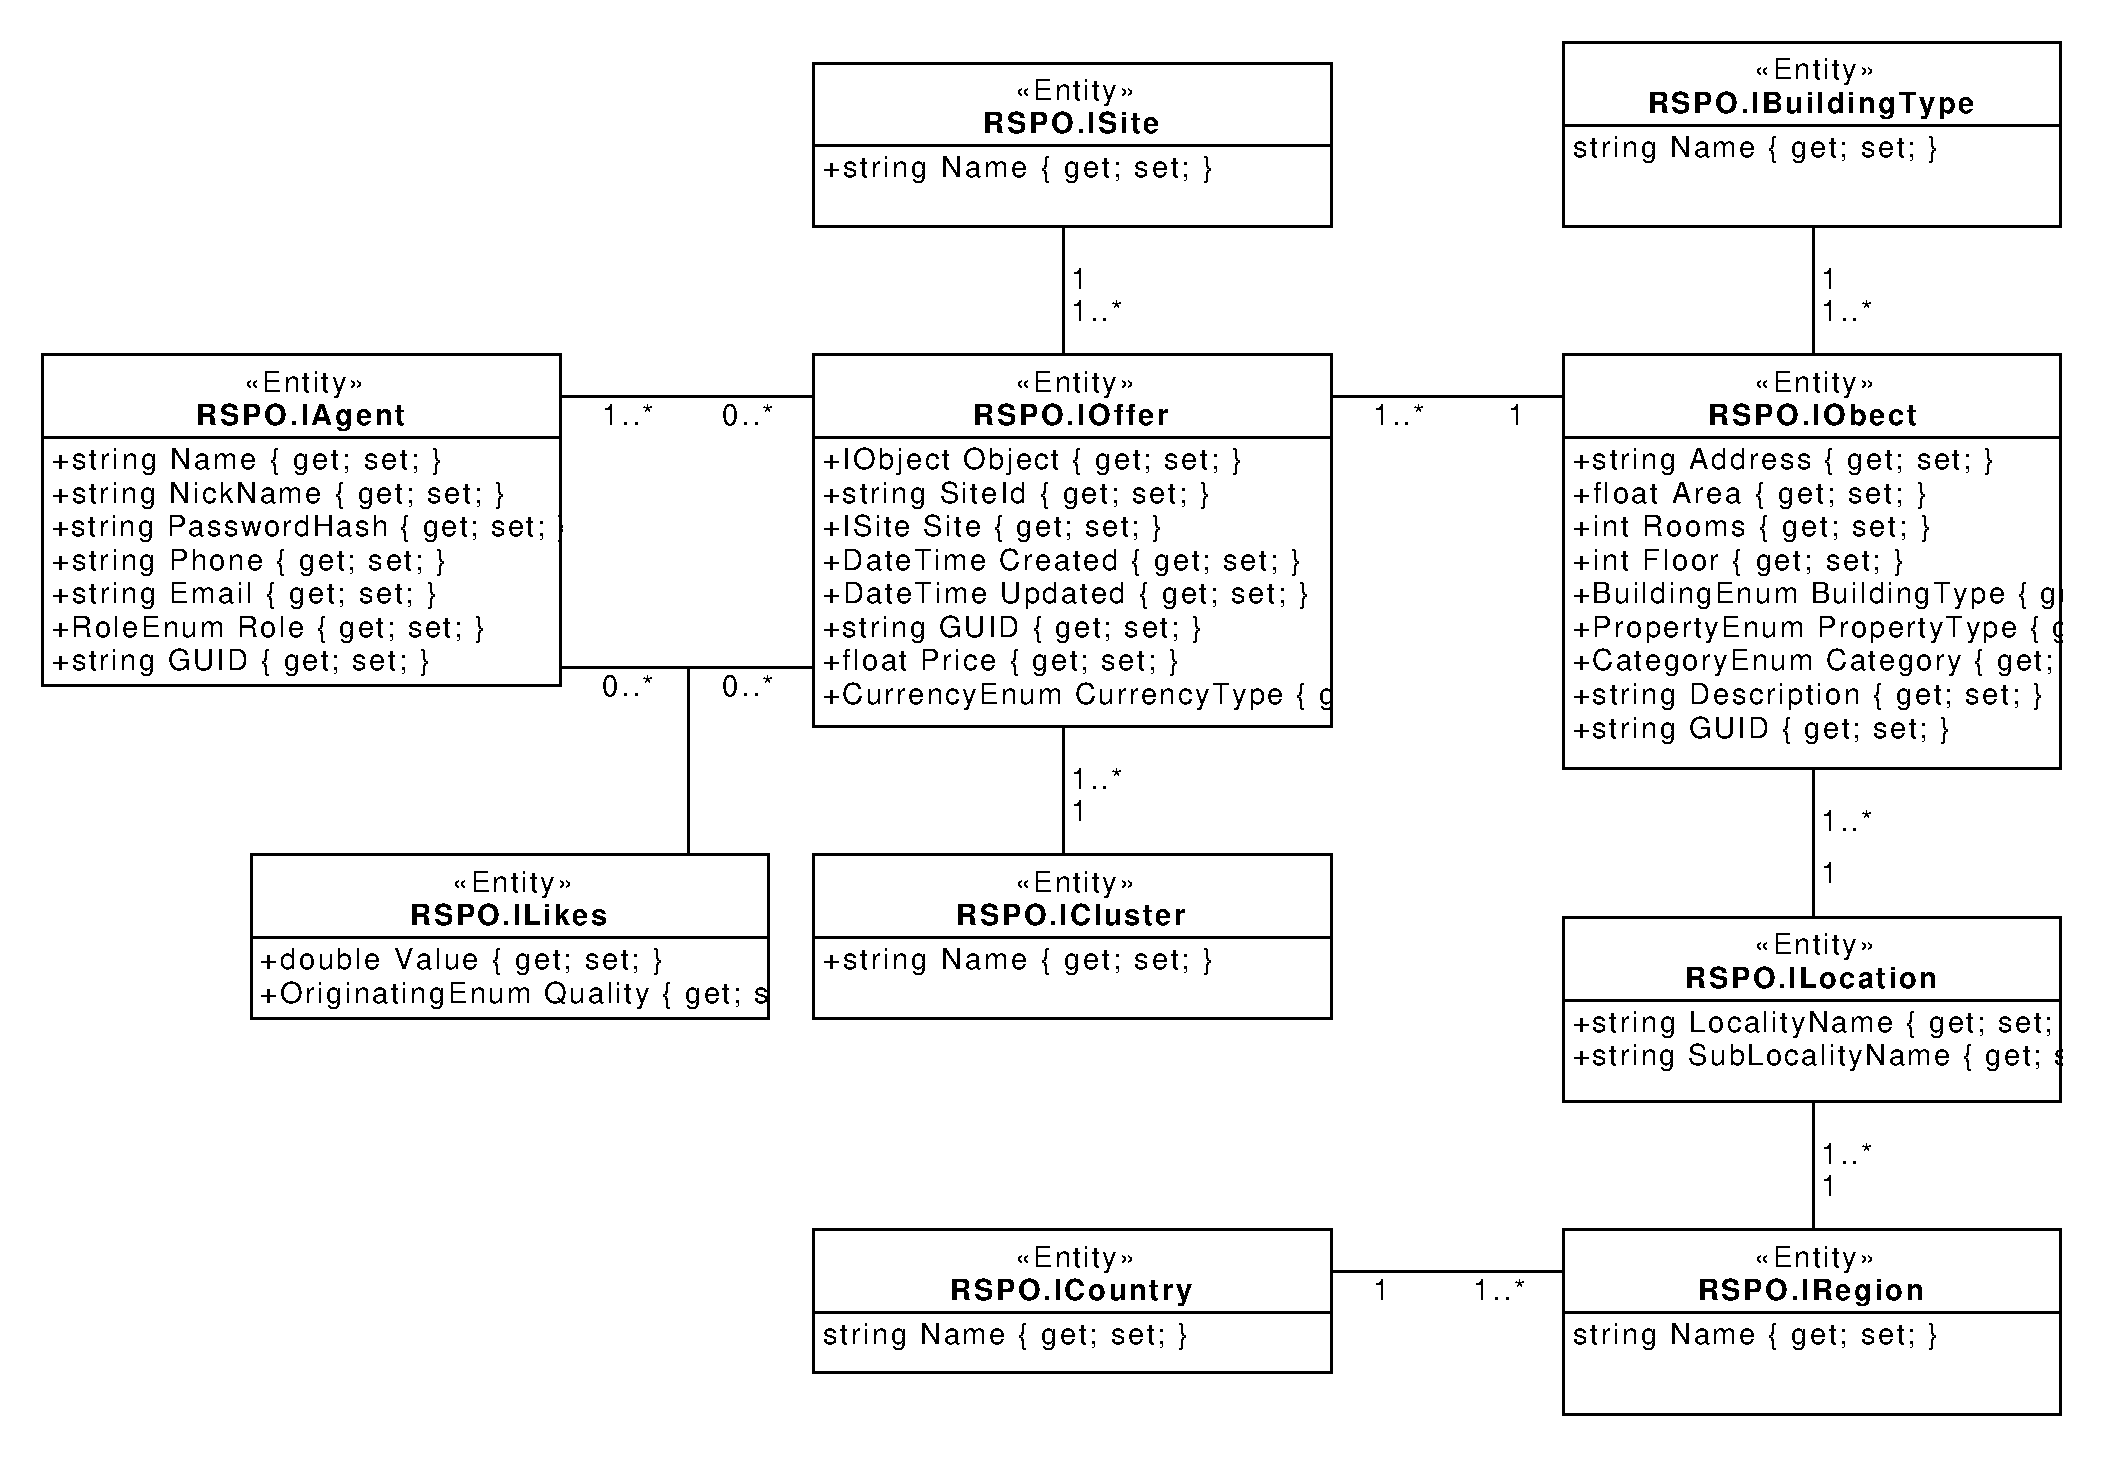
\includegraphics[width=1\linewidth]{class_diagram.pdf}
\end{frame}

\begin{frame}
  \frametitle{Screenshot: Naming clusters}
   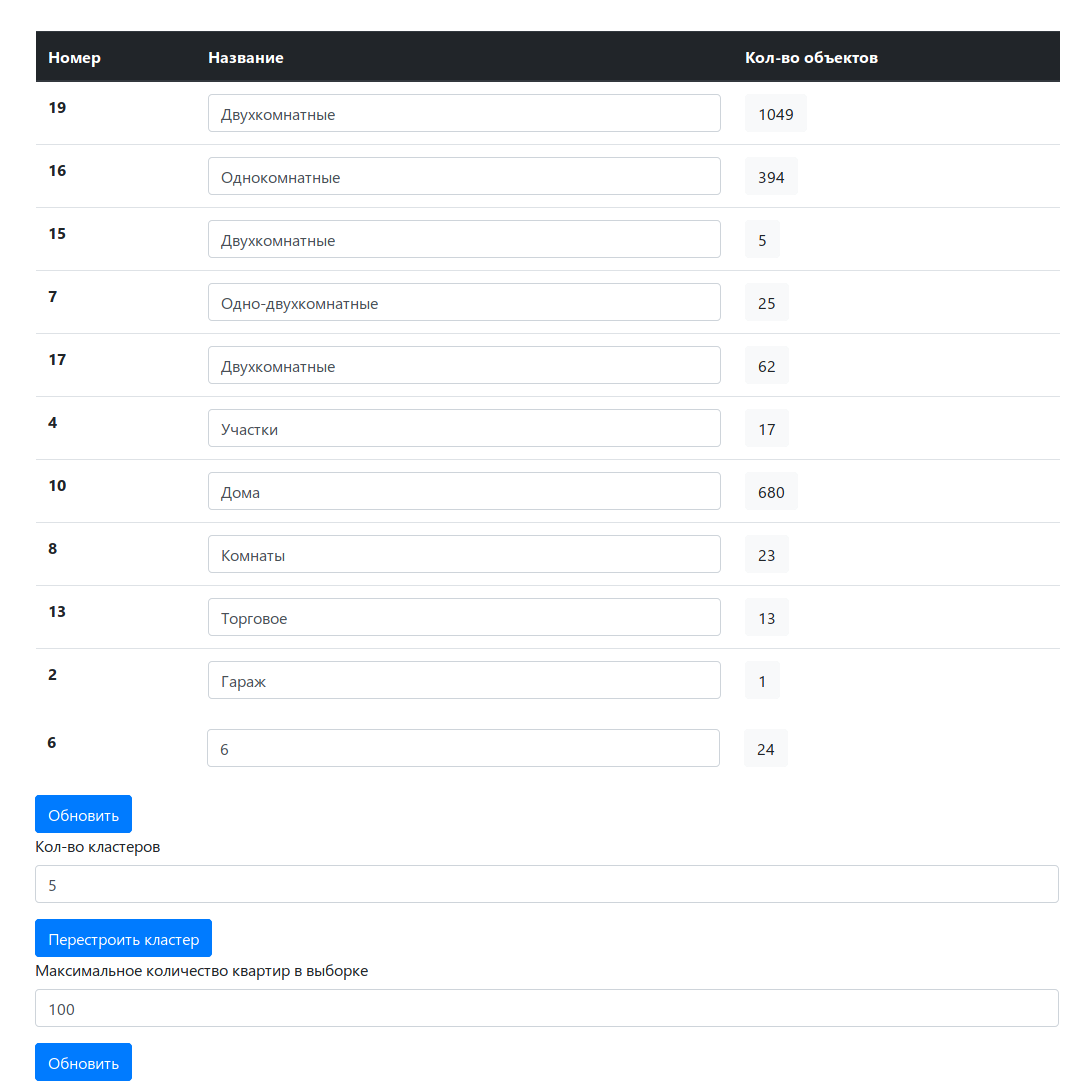
\includegraphics[width=1\linewidth]{screen-cluster.png}
\end{frame}

\begin{frame}
  \frametitle{Screenshot: Example of recommendation}
   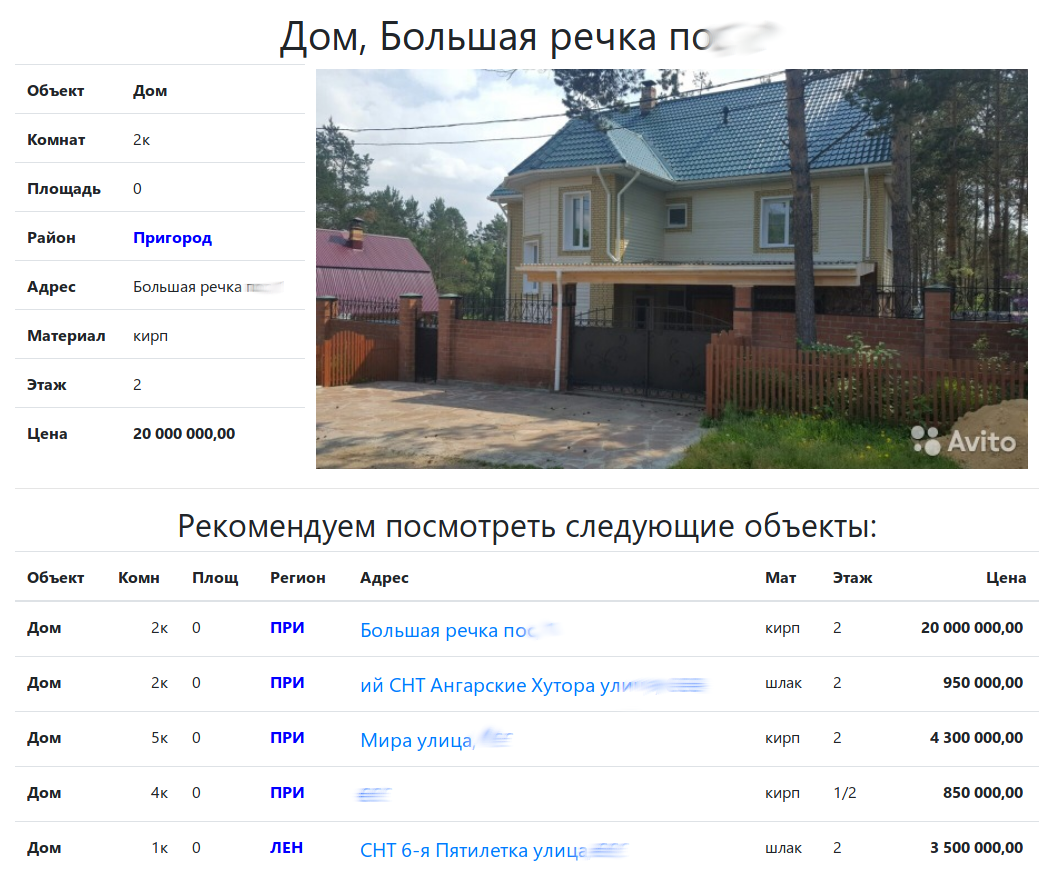
\includegraphics[width=1\linewidth]{screen-recommends.png}
\end{frame}

\begin{frame}
  \frametitle{Data sources and preliminary processing for entrants' RS}
  \textbf{Social networks} are popular ways of self-expression for school students (entrants).  User's properties are the profile data and set of group and channel subscriptions represented with \textbf{tags, keywords}.  TSU\footnote{Tomsk state university} research proved that InContact (ВКонтакте) students profiles are closely related to educational interests.

  To produce recalculations we make clusters of users and find ones, who has chosen a specialty.  Specialty data is extracted from \emph{enrollment orders}, which structure is regular.  Specialties described by competence relations are also organized in clusters, named by experts.

  Recommendations are to be produced with machine learning. \emph{e.g.}, a neural network (NN), pretrained to relate user class to a specialty [class].  Another NN will be used to distribute new entrants to classes.

  So the RS is based on \emph{content filtering}, and users will participate in RS functioning passively.
\end{frame}

\begin{frame}
  \frametitle{The summary of used technologies}

  \begin{itemize}
  \item \texttt{C\#} platform as compromise of expressiveness and performance, cross-platform (\texttt{.NET} and \texttt{MONO});
  \item Entity Framework (ET) for object persistency;
  \item \texttt{SQLEXPRESS} and \texttt{BrightstarDB} as ET backends with aim to RDF and LOD;
  \item \texttt{Microsoft.Office.Interop.Word} for DOCX processing;
  \item \texttt{HtmlAgilityPack} for HTML parsing;
  \item \texttt{dotNetRdf}, \texttt{System.Xml.Xdocument};
  \item \texttt{VDS.Common} for word indexing;
  \item \texttt{SharpTAL} for \texttt{HTML} templating;
  \item \texttt{Newtonsoft.Json} for \texttt{JSON} generation/parsing;
  \item \texttt{BCrypt} for user password encryption;
  \item \texttt{xunit.*} for organizing functional tests;
  \item \texttt{Paket} \texttt{.NET} dependency manager;
  \item Browser \texttt{JavaScript} with \texttt{Bootstrap} and \texttt{JQuery}.
  \end{itemize}
\end{frame}

\begin{frame}
  \frametitle{Discussion}
  The realty RS was tested by a number of buyers, none of them mentioned misbehavior of the system like spontaneous transitions from one class to another, or supplying empty sets of recommendations.

The presented experience shows that C\# .NET and MONO technologies and used techniques are well suitable for construction RS:
\begin{enumerate}
\item working in ``cold start'' conditions;
\item do not require user to register and authorize while implicit gathering information needed for recommendation generation;
\item testing systems are to be done in a local conditions to be able to check the results comparing with existing ``natural'' data;
\item using open-source technologies, modules and libraries.
\end{enumerate}

The obtained real estate RS implementation as well as the second project do not take advantage of the nowadays methods of R\&D development, which corresponds to current traditions.  Most attention is paid to preliminary data processing and obtaining minimal valuable product (MVP).
\end{frame}

\begin{frame}
  \frametitle{Conclusion}
  We presented results of two master degree projects.  The first one is finished, and the second one is on a half way.  Both systems have similar design, but rely on different RS techniques. Both systems use persistent object-oriented representation of application entities.

We have to solve ``cold start'' problem for both domains by creating taxonomies to consider classes as objects of users' interests.  Taxonomies of users are also created in Entrants' RS.

The techniques could be developed further by adaptation the standard directions such as:
\begin{itemize}
  \item usage of ontologies describing domain to extend search capabilities especially in students' courses domain;
  \item case based reasoning for the same domain;
  \item predictive modeling of attribute values for realty;
  \item providing geospacial data of infrastructural service organizations in the environment, \emph{e.g.} schools, kindergartens and shops.
\end{itemize}
\end{frame}


\begin{frame}{}
  \vfill
  \centering
  \Huge \textbf{Thank You for attention!}
  \vfill
  
\includegraphics[width=0.5\linewidth]{QRURL.png}\\
  \normalsize\url{https://github.com/eugeneai/papers-aiit-rs/raw/master/talk-2020-10-16-RS.pdf}
\end{frame}

\end{document}


%%% Local Variables:
%%% mode: latex
%%% TeX-master: "talk-2020-09-03-proposal.tex"
%%% End:
